\documentclass[10pt,a4paper]{article}
\usepackage[utf8]{inputenc}
\usepackage[german]{babel}
\usepackage{mathrsfs}
\usepackage{amsmath}
\usepackage{amsfonts}
\usepackage{amssymb}
\usepackage{amsthm}
\usepackage{graphicx}
\usepackage{float}
\usepackage[left=2cm,right=2cm,top=2cm,bottom=2cm]{geometry}

\begin{document}

\section{Aufgabe 1}

\section{Aufgabe 2}
Zuerst wird mit $10$ verglichen und danach schon mit $18$, was die Suche beendet und $6$ zurückgibt.

\section{Aufgabe 3}

\subsection{Sequentiell und Binär}
\begin{equation}
  k = 1
\end{equation}
\begin{equation}
  A_{1} = 1\ 2\ 3
\end{equation}
\begin{equation}
  A_{2} = 0\ 1\ 2
\end{equation}

\subsection{Sequentiell und Fibonacci}
\begin{equation}
  k = 1
\end{equation}
\begin{equation}
  A_{1} = 1\ 2\ 3\ 4
\end{equation}
\begin{equation}
  A_{2} = 0\ 1\ 2\ 3
\end{equation}

\subsection{Sequentiell und Interpolation}
\begin{equation}
  k = 100
\end{equation}
\begin{equation}
  A_{1} = 0\ 100\ 102\ 103\ 104\ 105\ 106\ 107
\end{equation}
\begin{equation}
  A_{2} = 99\ 100\ 101
\end{equation}

\subsection{Binär und Fibonacci}
\begin{equation}
  k = 4
\end{equation}
\begin{equation}
  A_{1} = 1\ 2\ 3\ 4\ 5\ 6\ 7
\end{equation}
\begin{equation}
  A_{2} = 2\ 3\ 4\ 5\ 6\ 7\ 8
\end{equation}

\subsection{Binär und Interpolation}
\begin{equation}
  k = 10
\end{equation}
\begin{equation}
  A_{1} = 0\ 5\ 10\ 50\ 100
\end{equation}
\begin{equation}
  A_{2} = 0\ 10\ 20\ 30\ 50
\end{equation}

\subsection{Fibonacci und Interpolation}
\begin{equation}
  k = 10
\end{equation}
\begin{equation}
  A_{1} = 0\ 1\ 10\ 11\ 12\ 13\ 70
\end{equation}
\begin{equation}
  A_{2} = 7\ 8\ 9\ 10\ 11\ 12\ 13
\end{equation}

\section{Aufgabe 4}
Die Schlüssel beginnen bei 1 und die X-Blätter habe ich eingefügt, um explizit anzuzeigen, dass die Suche auf der linken Seite erfolglos beendet wird.
\begin{figure}[H]
  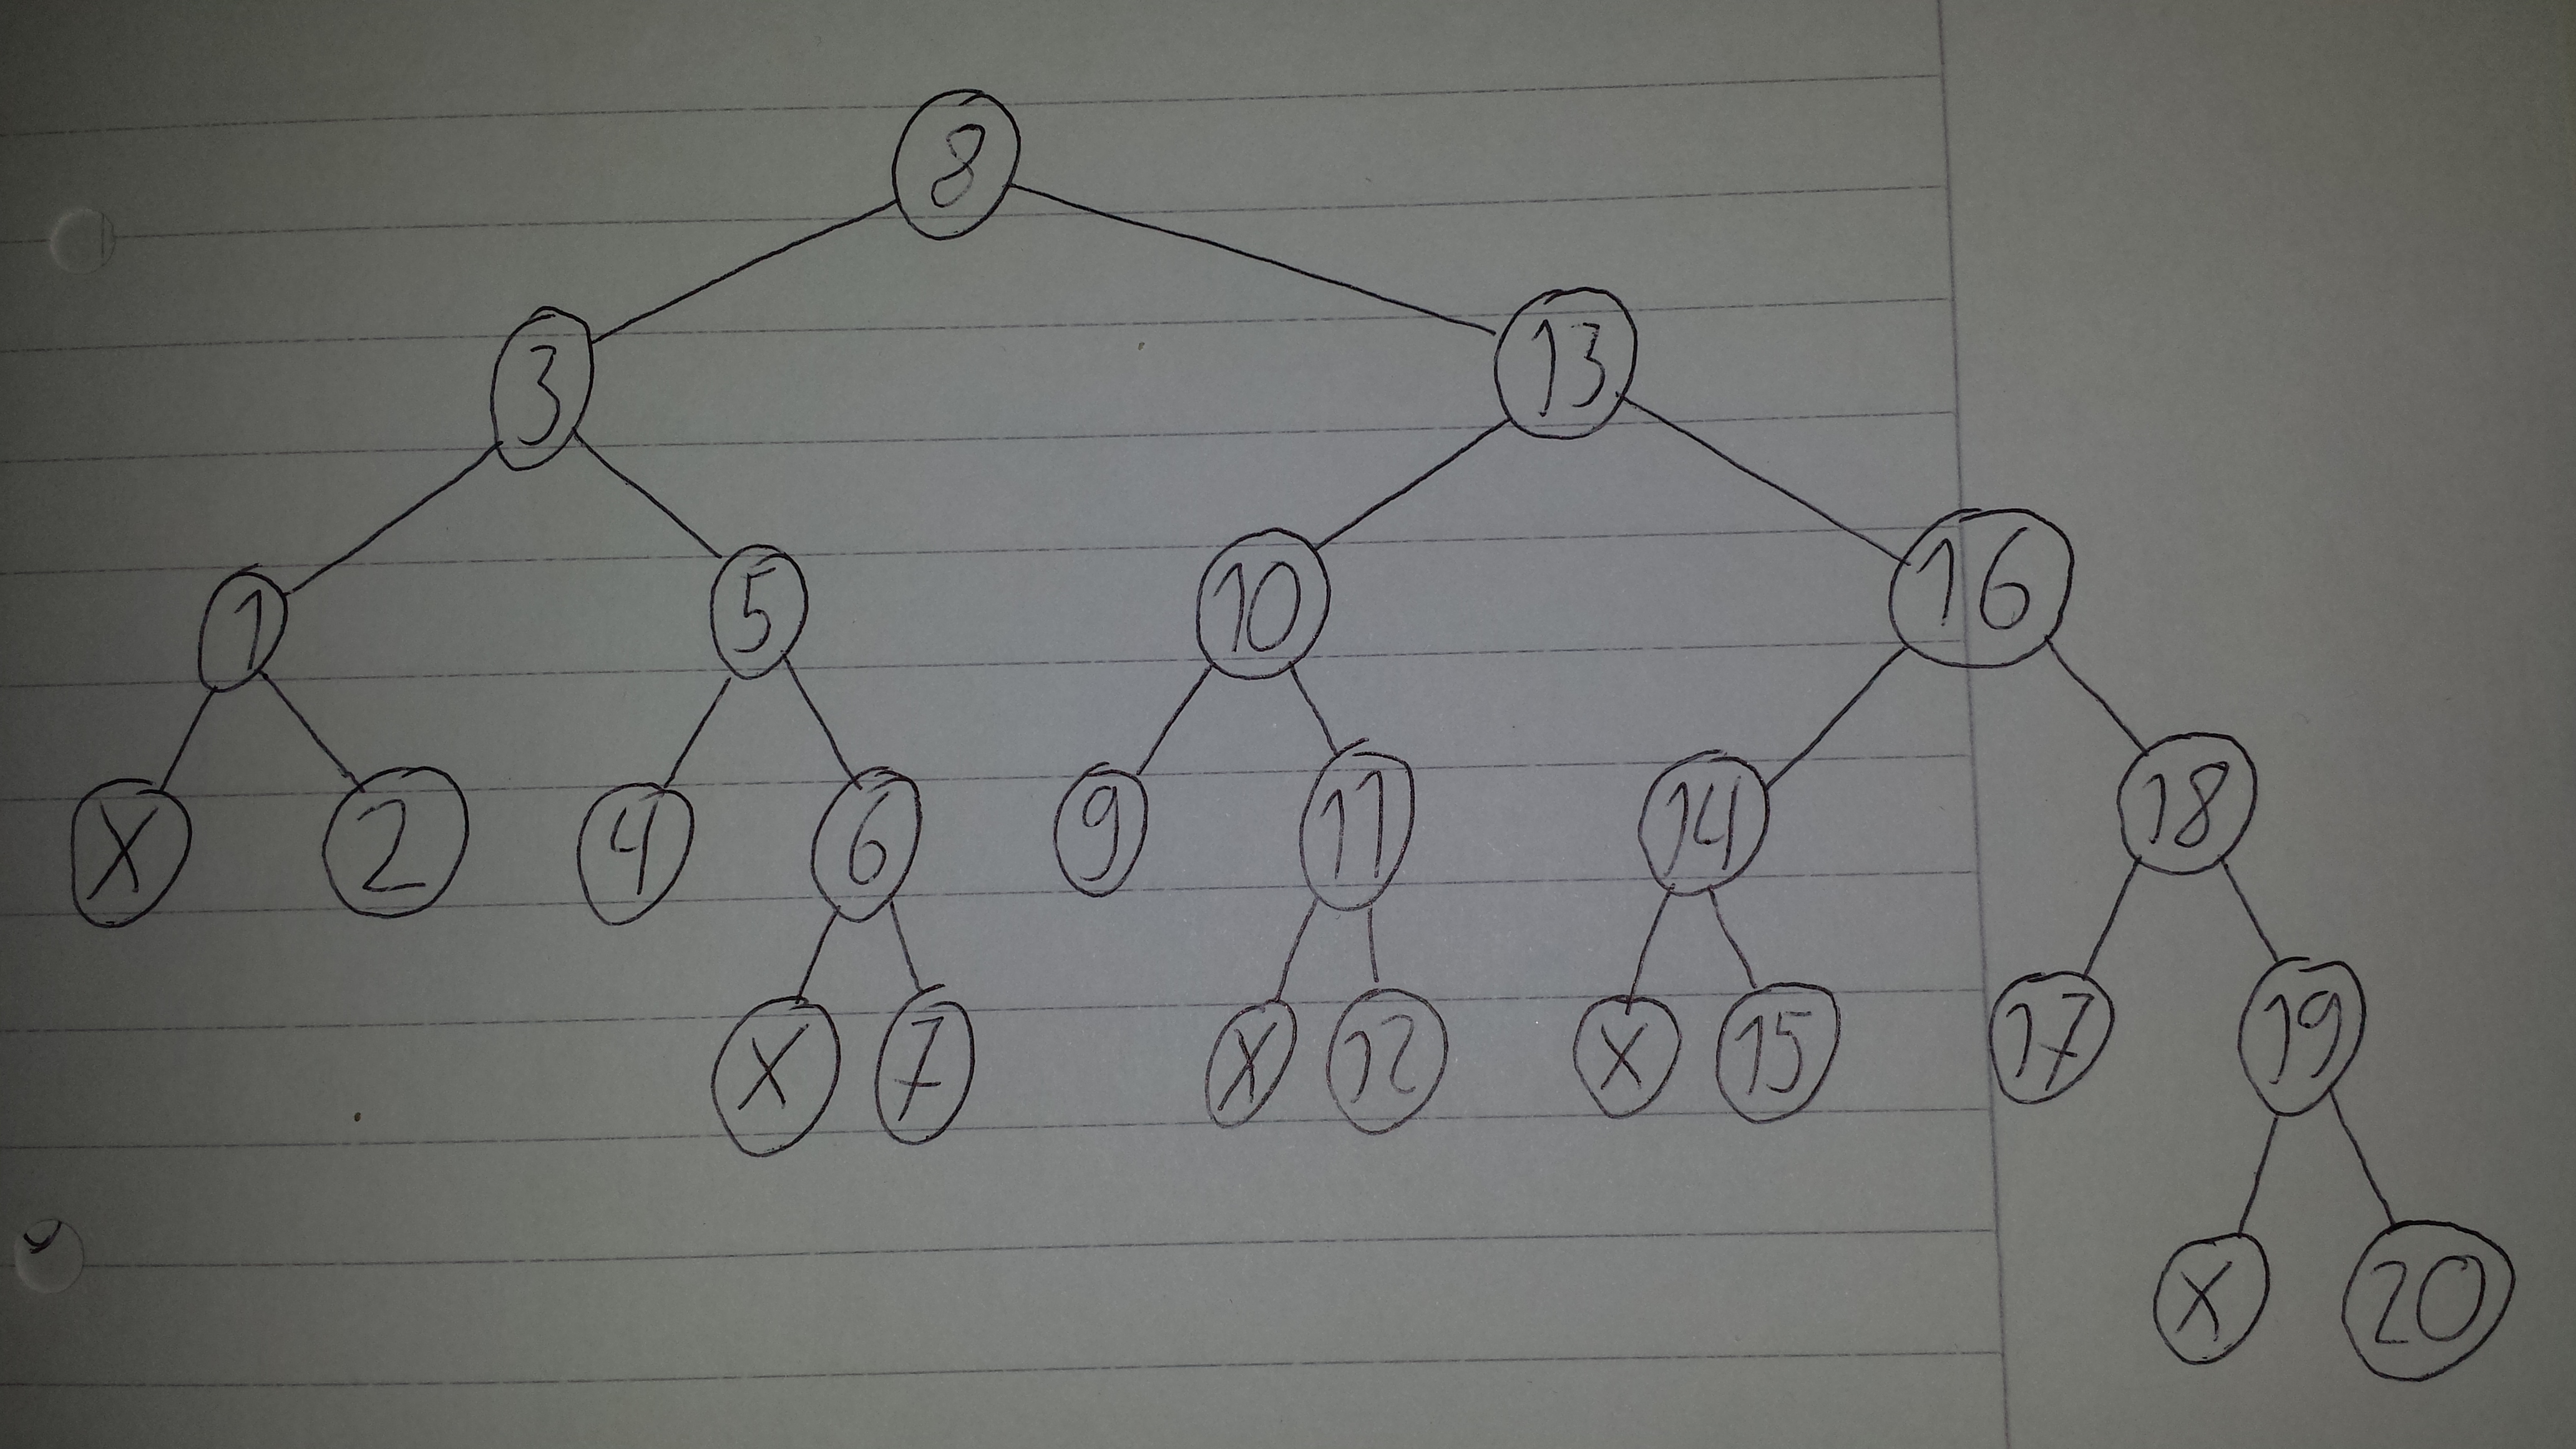
\includegraphics[width=400pt]{6_4}
\end{figure}

\end{document}